For X10 modtageren er der udviklet en række diagrammer ud fra applikationsmodel metoden.
På figur \ref{fig:X10_modtager_domain} er domænemodellen som resten af diagrammerne er udviklet ud fra.
Der er et sekvensdiagram på figur \ref{fig:X10_modtager_SD} for alle de aktuelle use-cases som beskriver systemets virkemåde.
Ud fra dette er der lavet et klassediagram på figur \ref{fig:X10_modtager_Class} som dækker de forskellige use-cases med controller klasser og kommunikationenen til CSS hovedenheden via X10.


\begin{figure}[!htb]
\centering 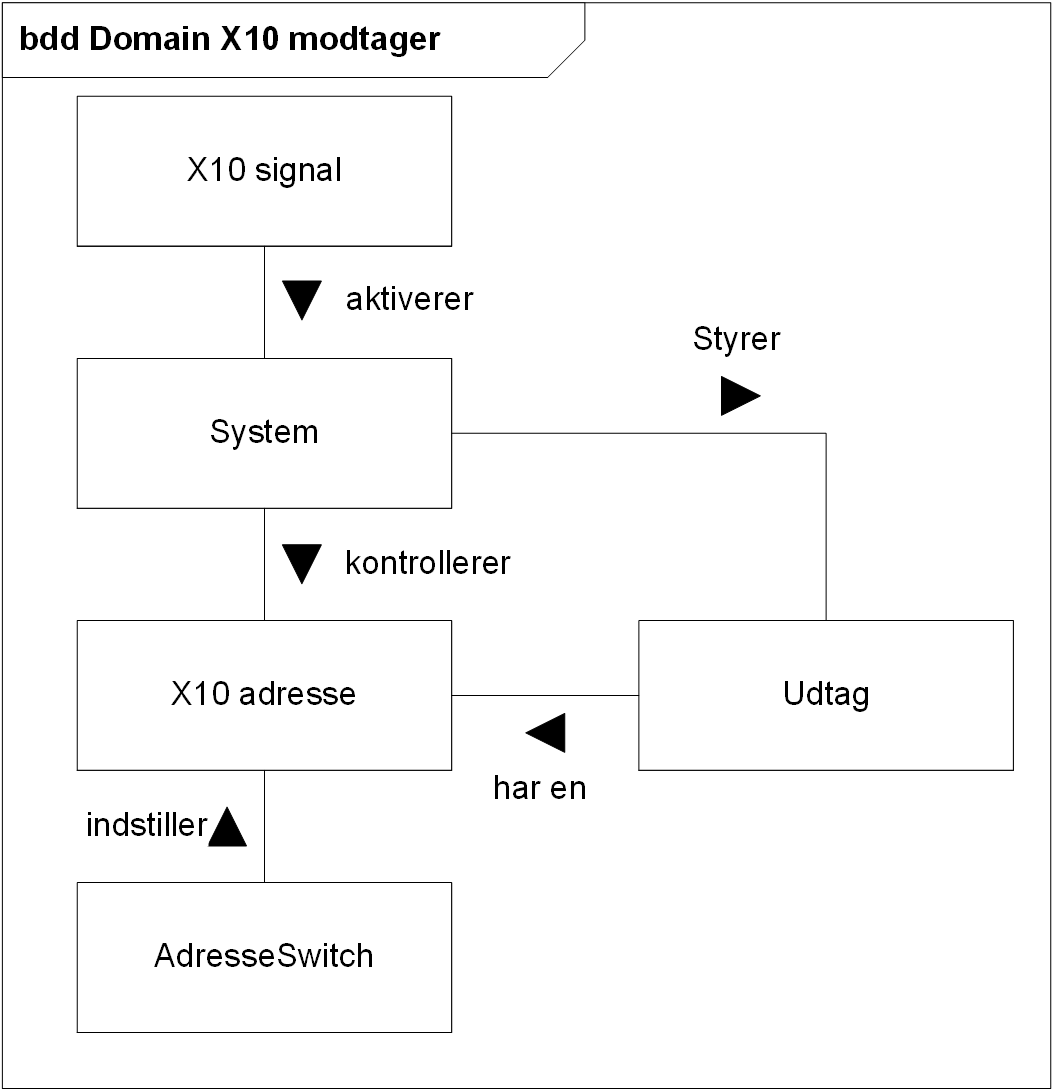
\includegraphics{billeder/uml/X10_modtager_Domain}
     \caption{Domænemodel for X10 modtager}
     \label{fig:X10_modtager_domain}
\end{figure}

\begin{figure}[!htb]
	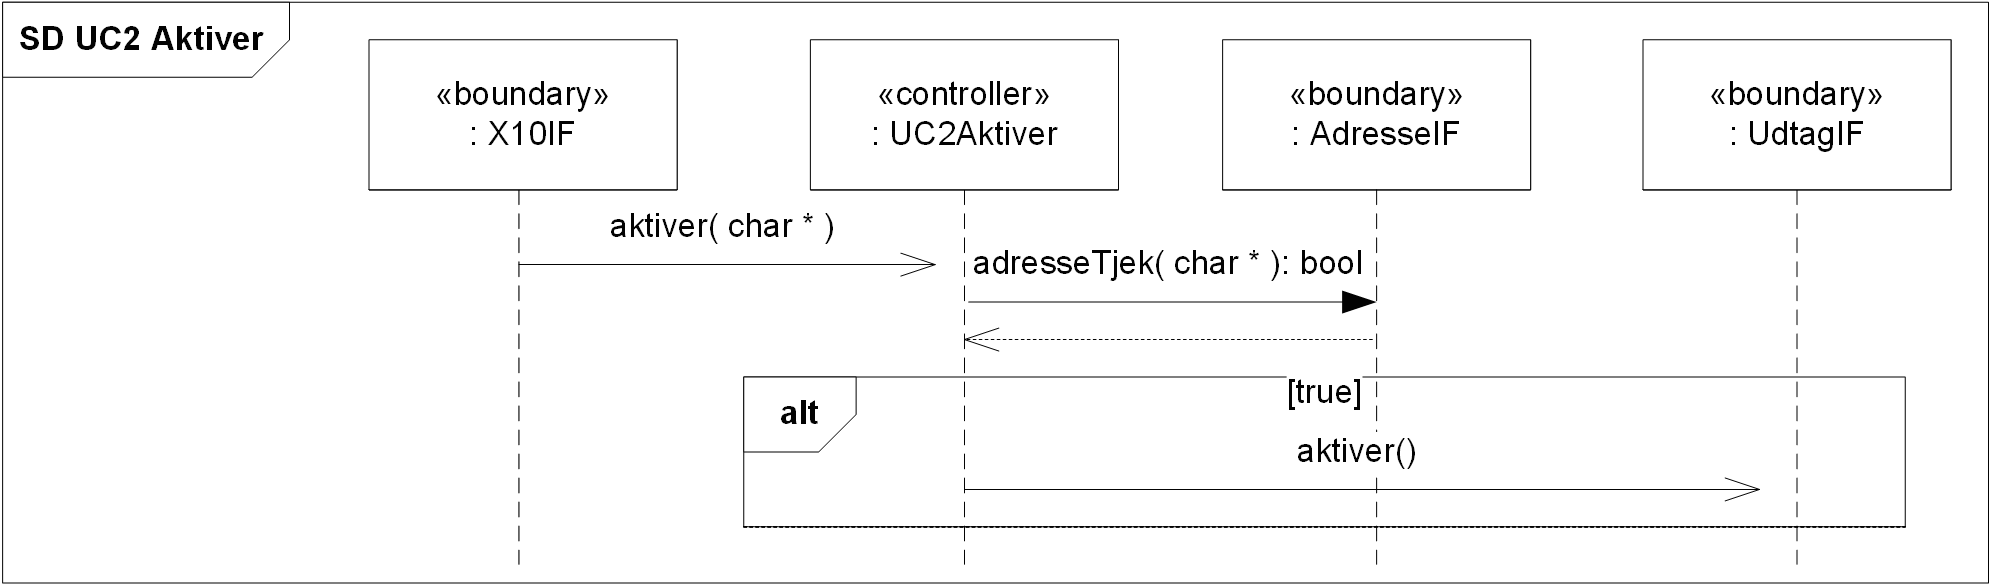
\includegraphics{billeder/uml/X10_modtager_SD}
     \caption{Use-case sekvensdiagrammer for X10 modtager}
     \label{fig:X10_modtager_SD}
\end{figure}

\begin{figure}[!htb]
     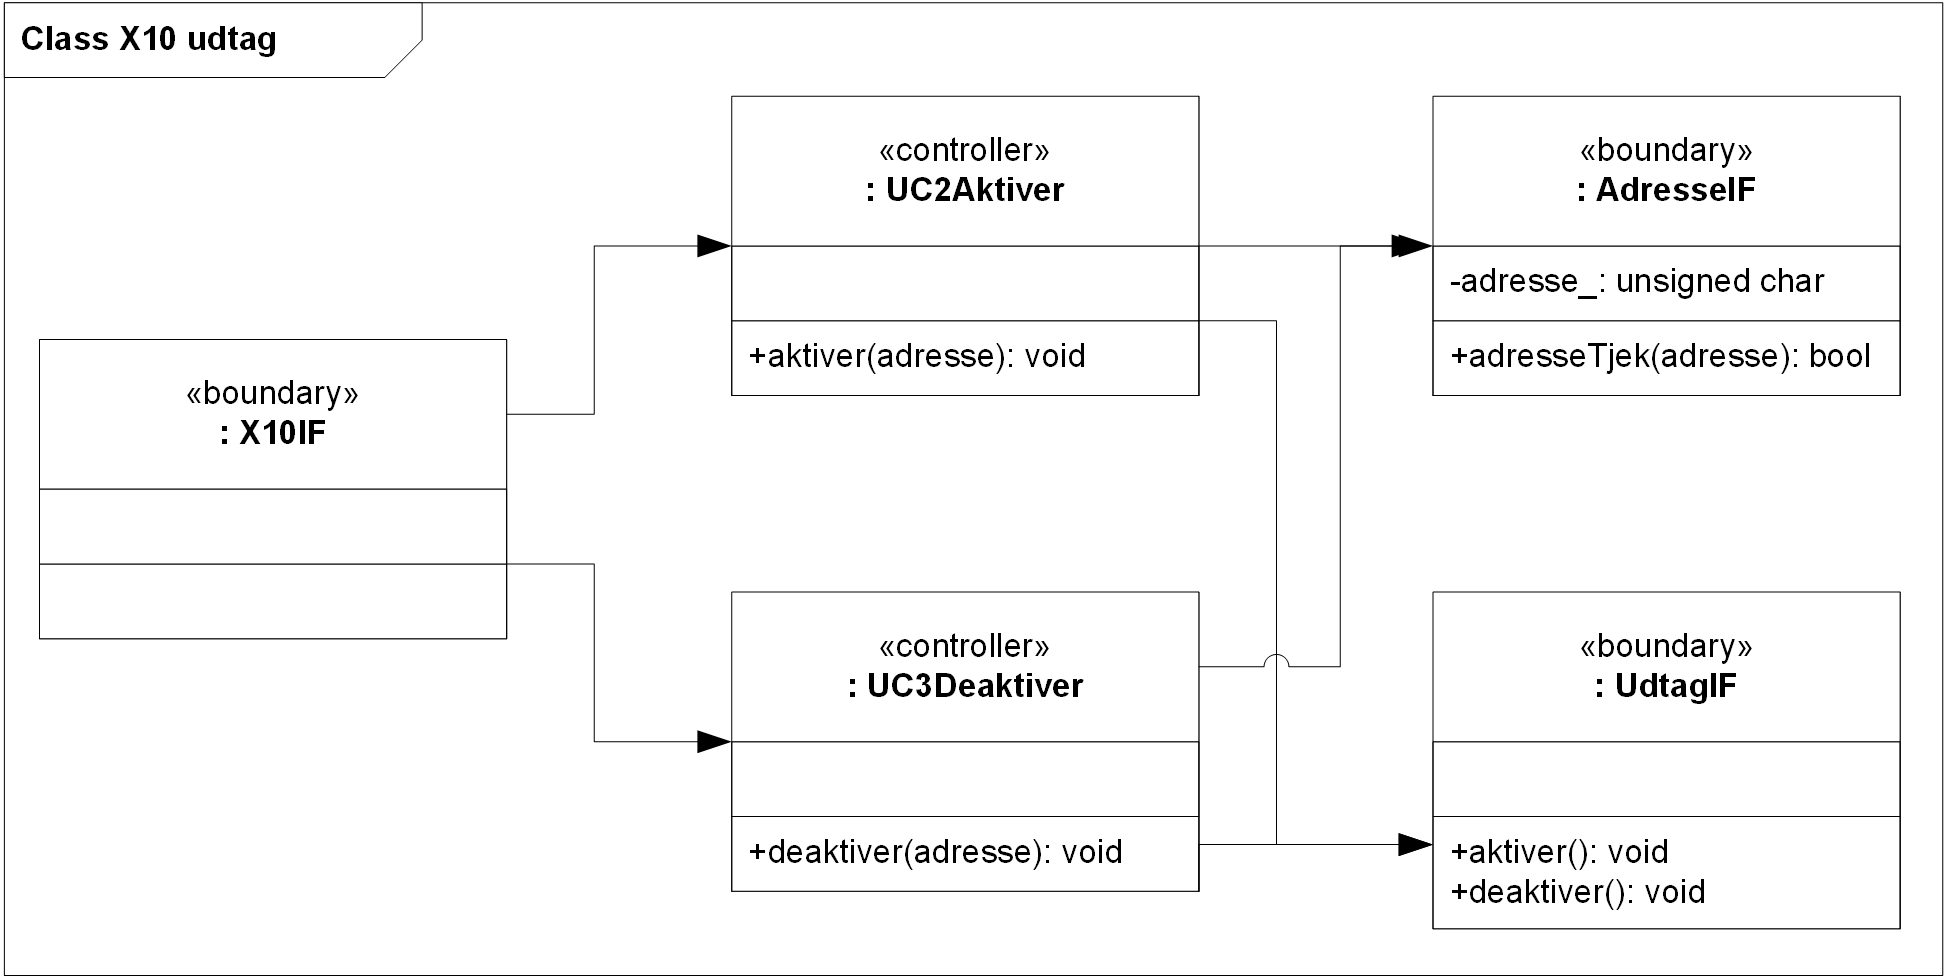
\includegraphics{billeder/uml/X10_modtager_Class}
     \caption{Klassediagram for X10 momdtager}
     \label{fig:X10_modtager_Class}
\end{figure}
